\section{Model}
This section presents, with theory, a comparison of two estimators for the mean of a collection of graphs by observing the adjacency matrices.  This work considers the scenario of having $M$ graphs represented as adjacency matrices, $\{A^{(m)}\}$ ($m = 1, \cdots, M$), each having $N$ vertices with known correspondence.  The graphs we consider are undirected and unweighted with no self-loops, i.e. each $A^{(m)}$ is a binary symmetric matrix with zeros along the diagonal. An example scenario of this arises in the field of connectomics, where functional brain imaging data for each subject can be represented as a graph, with each vertex having a defined anatomical correspondence, and an edge between two regions is defined to exist if correlation in activity between the regions reaches a certain threshold. In this setting, we consider each random graph to be sampled from the independent edge model with parameter $P \in [0,1]^{N\times N}$, where each edge between vertex $i$ and vertex $j$ exists independently with probability $P_{ij}$. We aim to estimate the probability matrix $P$ with our observations of the adjacency matrices $\{A^{(m)}\}$ of $M$ graphs.



\subsection{Entry-Wise Least Squares Estimate}
The most intuitive approach in this scenario is the element-wise mean among the adjacency matrices:
\begin{equation}
\bar{A} = \frac{1}{M}\sum\limits_{m = 1}^M A^{(m)}
\end{equation}
Since each element of the adjacency matrix $A_{ij}$ is a sample from the Bernoulli distribution with probability $P_{ij}$, with each element examined in isolation, to estimate the mean graph $P$ one would like to use the element-wise MLE, i.e. the element-wise mean, $\bar{A}$. Meanwhile, it is also the entry-wise least squares estimates.



\subsection{Random Dot Product Graph}
Hoff et. al. (2002) \cite{hoff2002latent} proposed a model for random graphs called Latent Positions Graph Model. In this model, each vertex $i$ has an associated latent vector $x_i \in \mathbb{R}^d$ (generally $d$ is much smaller than the number of vertices $N$), and the probability of a edge being present between two vertices only depends on their latent vectors through a link function. 

A specific instance of this model that we will examine is the random dot product graph model (RDPG) in which the link function is the dot product, i.e. the probability of an edge being present between two nodes is the dot product of their latent vectors. \cite{scheinerman2010modeling}. For example in the functional connectomics, components of the latent vectors may refer the relative importance of an anatomical region among a set of tasks.  The magnitude then may refer to how active the region is generally.  Therefore, active regions vital for a similar task are more likely to be functionally connected.

\subsection{Stochastic Block Model as a Random Dot Product Graph}
Generally, in a large graph, vertices are clustered into different communities such that vertices within the same community behave similarly. Such structural property is captured by the stochastic block model (SBM), where each vertex is assigned to a block and the probability that an edge exists between two vertices depends only on their respective block memberships. This imposes the idea of structural equivalence, where vertices are defined to be structurally equivalent if their connections to other nodes are similar.  In the stochastic block model, groups of vertices, or blocks, are then structurally equivalent since the vertices contained have equal likelihood in their connections among the blocks.  An example of block structure can be thought to exist in functional brain imaging, for instance the structures in the basal ganglia will likely behave similarly in their connections and may be considered a block.

Formally, the SBM is determined by the number of blocks $K$ (generally way less than the number of vertices $N$), block proportion vector $\rho$, and block probability matrix $B$. In this model each vertex is assigned to one of $K$ blocks and the fraction of vertices belonging to the $i$ th block is designated as $\rho_i$.  The connection probabilities of this block structure are stored in the symmetric $K \times K$ block matrix $B$, where $B_{ij}$ represents the probability of an edge existing between a vertex of block $i$ and one of block $j$.

\begin{figure}[!htb]
	\centering
	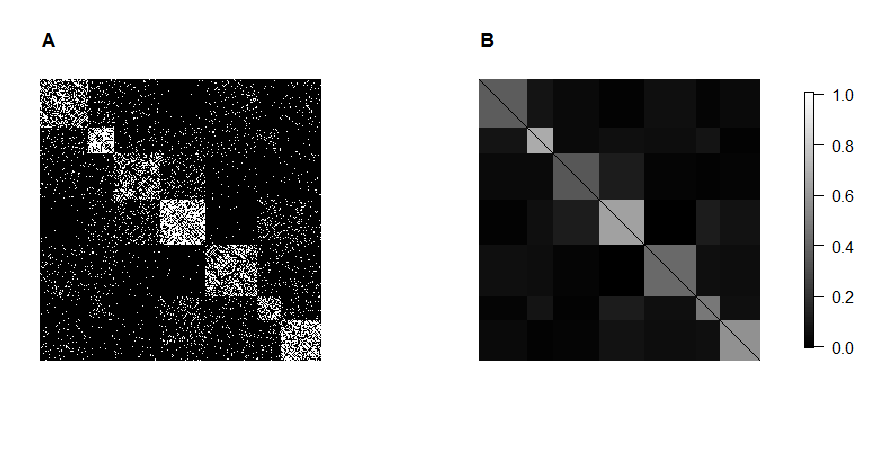
\includegraphics[width=16cm]{SBM_Example.png}
	\caption{Example illustrating the SBM. (a) Probability matrix that follows a SBM with K = 7 blocks; (b) Adjacency matrix generated from the SBM with probability matrix in (a).
	\label{fig:plot1}
\end{figure}


Now if we consider the SBM as a random dot product graph, all vertices in the same block would have identical latent positions.



\subsection{Estimator $\hat{P}$ Based on Adjacency Spectral Embedding}
In order to take advantage of the underlying low dimensions of the RDPG,  we would like to use the adjacency spectral embedding (ASE) studied by Sussman et. al. to enforce a low rank approximation on the adjacency matrix $A$, which will decrease the variance if we embed it into the right dimension \cite{sussman2012consistent}.  The adjacency spectral embedding creates an approximated RDPG representation of the adjacency matrix from its low rank eigen-decomposition.  The latent vectors are stored as a $N \times d$ matrix $X$, where the columns are comprised of the eigenvectors associated with the $d$ largest eigenvalues of the adjacency matrix. Then $X_i$, each row of $X$, is a latent vector for the corresponding vertex $i$.

In this work, rather than stopping at the element-wise MLE $\bar{A}$, we use ASE to embed the mean matrix $\bar{A}$ to $X$ and then take $\hat{P} = X X^T$ as our estimate for $P$.  Due to the underlying block-distibuted RDPG structure of graphs, enforcing this low rank approximation on $\bar{A}$ will provide a better estimate for the true mean matrix $P$.  Details of this algorithm are presented in Section \ref{subsection:alg}.

\subsection{Performance Evaluation: Relative Efficiency}
To compare the performance between $\hat{P}$ and $\bar{A}$, we examine the relative efficiency (RE), in mean squared error (MSE), among the two defined as:
\begin{equation}
RE_{ij} = \frac{MSE(\hat{P}_{ij})}{MSE(\bar{A}_{ij})}
\end{equation}
